\PassOptionsToPackage{unicode=true}{hyperref} % options for packages loaded elsewhere
\PassOptionsToPackage{hyphens}{url}
%
\documentclass[11pt,]{article}
\usepackage{lmodern}
\usepackage{amssymb,amsmath}
\usepackage{ifxetex,ifluatex}
\usepackage{fixltx2e} % provides \textsubscript
\ifnum 0\ifxetex 1\fi\ifluatex 1\fi=0 % if pdftex
  \usepackage[T1]{fontenc}
  \usepackage[utf8]{inputenc}
  \usepackage{textcomp} % provides euro and other symbols
\else % if luatex or xelatex
  \usepackage{unicode-math}
  \defaultfontfeatures{Ligatures=TeX,Scale=MatchLowercase}
\fi
% use upquote if available, for straight quotes in verbatim environments
\IfFileExists{upquote.sty}{\usepackage{upquote}}{}
% use microtype if available
\IfFileExists{microtype.sty}{%
\usepackage[]{microtype}
\UseMicrotypeSet[protrusion]{basicmath} % disable protrusion for tt fonts
}{}
\IfFileExists{parskip.sty}{%
\usepackage{parskip}
}{% else
\setlength{\parindent}{0pt}
\setlength{\parskip}{6pt plus 2pt minus 1pt}
}
\usepackage{hyperref}
\hypersetup{
            pdftitle={Statistics : Correlation coefficient},
            pdfborder={0 0 0},
            breaklinks=true}
\urlstyle{same}  % don't use monospace font for urls
\usepackage[margin=1in]{geometry}
\usepackage{longtable,booktabs}
% Fix footnotes in tables (requires footnote package)
\IfFileExists{footnote.sty}{\usepackage{footnote}\makesavenoteenv{longtable}}{}
\usepackage{graphicx,grffile}
\makeatletter
\def\maxwidth{\ifdim\Gin@nat@width>\linewidth\linewidth\else\Gin@nat@width\fi}
\def\maxheight{\ifdim\Gin@nat@height>\textheight\textheight\else\Gin@nat@height\fi}
\makeatother
% Scale images if necessary, so that they will not overflow the page
% margins by default, and it is still possible to overwrite the defaults
% using explicit options in \includegraphics[width, height, ...]{}
\setkeys{Gin}{width=\maxwidth,height=\maxheight,keepaspectratio}
\setlength{\emergencystretch}{3em}  % prevent overfull lines
\providecommand{\tightlist}{%
  \setlength{\itemsep}{0pt}\setlength{\parskip}{0pt}}
\setcounter{secnumdepth}{0}
% Redefines (sub)paragraphs to behave more like sections
\ifx\paragraph\undefined\else
\let\oldparagraph\paragraph
\renewcommand{\paragraph}[1]{\oldparagraph{#1}\mbox{}}
\fi
\ifx\subparagraph\undefined\else
\let\oldsubparagraph\subparagraph
\renewcommand{\subparagraph}[1]{\oldsubparagraph{#1}\mbox{}}
\fi

% set default figure placement to htbp
\makeatletter
\def\fps@figure{htbp}
\makeatother

\usepackage{longtable}
\usepackage{hologo}
\LTcapwidth=.95\textwidth
\linespread{1.05}
\usepackage{hyperref}

\title{Statistics : Correlation coefficient}
\author{true \and true \and true}
\date{May 23, 2021}

\begin{document}
\maketitle

\hypertarget{introduction}{%
\section{Introduction}\label{introduction}}

As an apogee of the introduction to statistics course and top off the
final moments of being a first year undergraduate in International
Relations, this project reflects all the knowledge acquired throughout
the past few months of this introductory class. Beginning with no
history in programming nor experience in writing a scientific report on
Rmarkdown, we were able to learn and develop step by step, our insight
on the `magic' of Data Analytics.

We are grateful to have had the chance to receive a rather large glance
at basic R commands and to put into practice the notions seen during the
classes. Now, we are pleased to lead you through the outcome resulting
from our small but still progressing abilities in statistics.

\hypertarget{description-of-the-task}{%
\section{Description of the task}\label{description-of-the-task}}

In question 1 of exercise 2, our topic is related to bias study, non
linear relationship. We are asked to draw samples from a PDF for (X,Y),
where (X, Y) have a nonlinear relationship, using the function
gen\_nonlinear. Using the parameters assigned to us as well as an angle
parameter, we had to explain how the angle parameter visually affect the
data by comparing two scatterplots, one when the data is generated with
angle = 0, and the other when the data is generated with angle = -0.45.

In question 2 of the same exercise, we study the Confidence Interval
Coverage. We are given the task to study the coverage of different
confidence intervals (CIs) for Px,y, in the following data settings: 1.
the PDF of (X,Y) is a bivariate normal PDF 2. the PDF of (X,Y) is a
bivariate normal PDF, but the observed sample contains outliers 3. the
PDF of (X,Y) is a discrete PDF 4. X and Y have a nonlinear relationship

The types of confidence intervals used are the parametric bootstrap CI
of level = 0.8 and the nonparametric bootstrap CI of level = 0.8. We
used

\hypertarget{motivation}{%
\section{Motivation}\label{motivation}}

We decided to take part in this scientific report as we wanted to apply
the numerous theoretical theories seen in the course provided by
Profesor Victoria-Feser. We also saw this project as an opportunity to
meet new people and experience the workgroup process, as we can combine
our knowledge and perspective on the matter while being able to discuss
within a group.

\hypertarget{analysis}{%
\section{Analysis}\label{analysis}}

\begin{figure}

{\centering 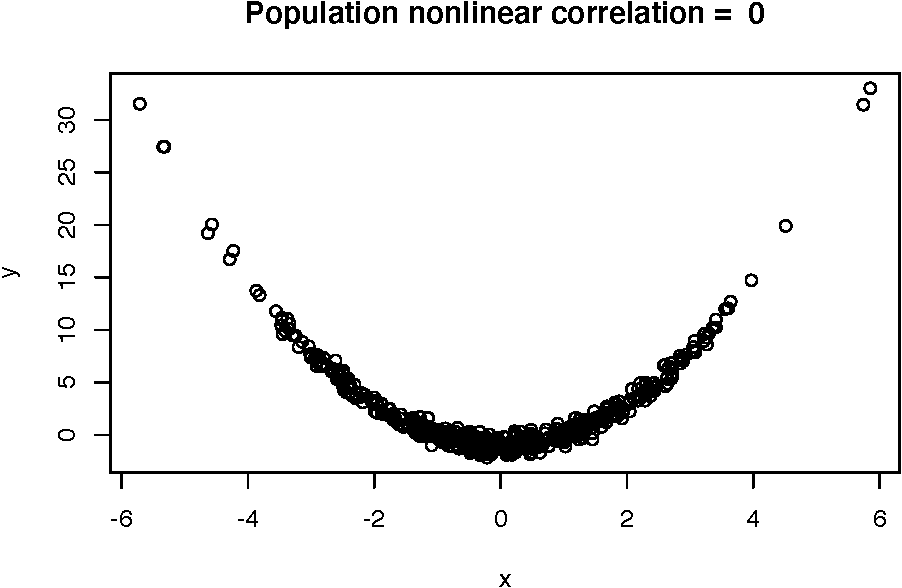
\includegraphics[width=0.5\linewidth]{RapportSTAT_files/figure-latex/nonlinear_q1-1} 

}

\caption{Hammock, this is the population correlation with angle = 0}\label{fig:nonlinear_q1}
\end{figure}

\begin{figure}

{\centering 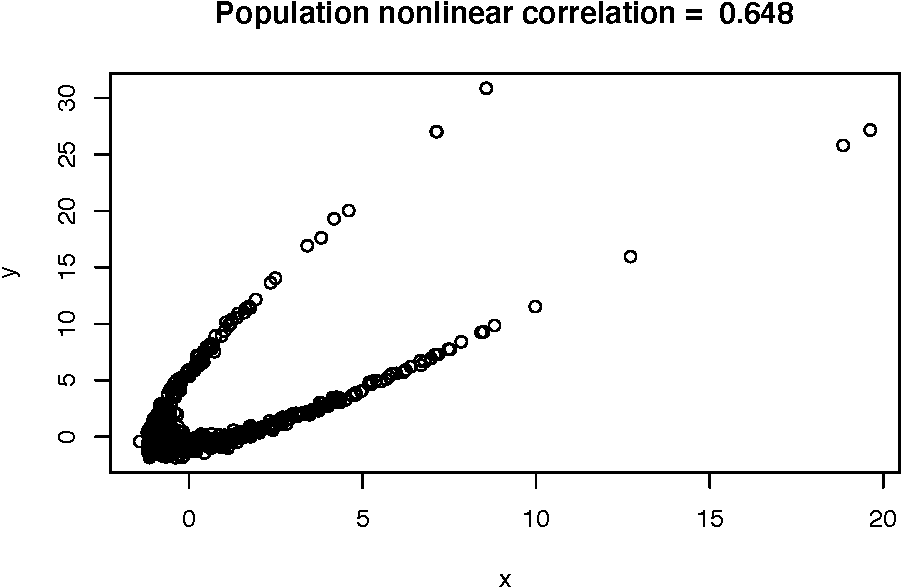
\includegraphics[width=0.5\linewidth]{RapportSTAT_files/figure-latex/nonlinear_q2-1} 

}

\caption{Comet, this is the population correlation with angle = -0.45}\label{fig:nonlinear_q2}
\end{figure}

Here we see the two scatterplots of when the data is generated with
angle = 0 (Hammock), and when it is generated with angle = -0.45 (Comet)
from the samples from a PDF of (X, Y), where (X,Y) have a nonlinear
relationship.

Hammock describes a positive relationship between X and Y as the graph
shows a convex parabola (x\^{}2). As we generate the data with an angle
parameter of -0.45, we see that there is a rotation to the left. Thus,
we deduce that the angle does visually affect the data, in that it
imposes a rotation.

Furthermore, when the angle moves from \(-\pi\) to \(+\pi\), we observe
a complete rotation of the parabola.

\hypertarget{results-and-discussion-description-and-interpretation-of-the-results}{%
\section{Results and discussion: description and interpretation of the
results}\label{results-and-discussion-description-and-interpretation-of-the-results}}

\begin{longtable}[]{@{}llrrrr@{}}
\toprule
& & Normal PDF & with outliers & Discrete PDF & Nonlinear
PDF\tabularnewline
\midrule
\endhead
parametric boot & n = 33 & 0.771 & 0.639 & 0.776 & 0.681\tabularnewline
& n = 110 & 0.783 & 0.257 & 0.776 & 0.63\tabularnewline
non-parametric boot & n = 33 & 0.758 & 0.758 & 0.753 &
0.725\tabularnewline
& n = 110 & 0.773 & 0.431 & 0.769 & 0.723\tabularnewline
\bottomrule
\end{longtable}

The parametric bootstrap, as it is implemented, assumes that the random
variables are bivariate normal.

How does it affect its performance, in terms of coverage, in the
different data settings? We observe a decrease in the interval
confidence when the parametric boot is performed on non parametric
functions such as the discrete and nonlinear, as seen in the blue data

In what data setting do you expect the nonparametric bootstrap to
perform better? We expect the nonparametric bootstrap to perform better
on a discrete PDF, as it is not a parametric function.

We assume from these obtained results, that the bivariate normal PDF
worked the best at approaching the confidence interval. We can see that
0.783 is the closest to 0.8, particularly when operating with the
parametric boot type.

We observe that the boot type parameter works the best when applied on a
normal PDF, as displayed by the green data. As the boot type parameter
is based on the mean and standard deviation, it is the most optimal
approach to compute the normal PDF's confidence interval as the latter
contains these two parameters. As for the non-parametric boot, it is the
most optimal when applied on a no parameter function like the nonlinear
function. It is displayed by the red data, which shows a greater
confidence interval than the blue data, computed with a parametric boot.

Then with the outliers setting, we see that as the n is larger, the
number of outliers increases, thus making the result further than the
confidence interval. The most surprising part of the table, is that the
difference between the outliers setting when n = 33 and when n = 110,
using the parametric boot type is quite large compared to when the data
is performed with the nonparametric boot type.

\hypertarget{statistical-methods-used}{%
\section{Statistical methods used}\label{statistical-methods-used}}

The Pearson method is used to calculate a correlation coefficient that
describes the strength relationship between two variables, in our case X
and Y, which ranges from 0 to 1. The closer the correlation coefficient
is to 0, the more the variables are independent from each other. When
equal to 1, the variables are equal to each other. The Pearson method
can be used on empirical observations in daily life. For instance, if we
want to evaluate whether there is a positive or negative relationship
between a student's age and their level of income when working at
Starbucks.

The Spearman rank correlation method is the nonparametric version of the
Pearson correlation coefficient method (``Lund Research Ltd'', 2018). It
is distinct in that the Spearman correlation coefficient is used to
determine the strength of a monotonic relationship, which is a type of
function that only increases or only decreases. In real life, we can
imagine that the Spearman method would be used to see whether an Unige
exam performance in Statistics is associated with the time students
spent studying in the UniMail library.

\hypertarget{acquired-skills-during-the-term-project}{%
\section{Acquired skills during the term
project}\label{acquired-skills-during-the-term-project}}

By accomplishing this report, we had an opportunity to broaden the use
of the R language by computing various aspects of the topics seen in
class. Despite a short learning period time, we are now able to compute
various functions on R and interpret codes. Furthermore, learning to
code has opened new perspectives as well as revealed numerous ways of
interpreting datasets. We will be able to apply these perspectives to
diverse daily socio-political situations. For these reasons, the present
report benefitted us greatly to acquire skills that will make our
International Relations studies more valuable.

\hypertarget{conclusion}{%
\section{Conclusion}\label{conclusion}}

In conclusion, in the Nonlinear Relationship Study, we see that the
angle parameter does affect the data by imposing a rotation, displacing
the parabola. As for the Confidence Interval Coverage Study, the
Confidence Interval of type npboot and of type boot results in different
outcomes depending on the setting and the sample size. Overall, most of
the outcomes are close to the confidence interval with a level = 0.8, as
one would expect.

via GIPHY

\hypertarget{you-can-scan-the-qr-code-with-you-mobile-phone-for-a-refreshing-surprise}{%
\subsubsection{You can scan the QR code with you mobile phone for a
refreshing
surprise!}\label{you-can-scan-the-qr-code-with-you-mobile-phone-for-a-refreshing-surprise}}

\end{document}
